% !TEX root = ./memoire/main.tex
% \section{Introduction}

% L'objectif de ce chapitre est de présenter les différentes entités nécessaires à la construction d'un jumeau numérique. Nous présenterons tout d'abord, quels sont les modélisations physiques utilisés pour simuler l'étape du broyeur à boulets. Nous traiterons uniquement la modélisation du mélange et de l'écoulement granulaire au sein du tambour en rotation. Dans un second temps, nous présenterons les méthodes d’acquisition utilisé pour . Finalement, nous présenterons la notion de jumeau numérique et présenterons dans quel cadre observation et simulation peuvent-ils être mis en relation.

\subsection*{Écoulement d'un milieu granulaire}~\label{sec:simu_granulaire}

La simulation du broyeur repose sur la représentation de l'écoulement d'un milieu granulaire. Si les écoulements granulaires sont très présents dans la nature et dans l'industrie, du fait de la nature discrète du milieu, ils sont bien moins comprise que l'écoulement d'un liquide qui se base sur les équations de Navier-Stokes.

L'écoulement granulaire va se distinguer par trois types de régime que l'on assimile aux trois états de la matière: solide où où le mouvement des particules est lent et le comportement est presque statique, une couche semblable à un liquide dans laquelle les grains s'écoulent avec une certaine inertie, et une zone semblable à un gaz où les particules se déplacent à des vitesses plus élevées de manière chaotique. Ils interviennent simultanément dans l'écoulement. Ce qui complexifie sa caractérisation rhéologique.
\begin{figure}
    \centering
    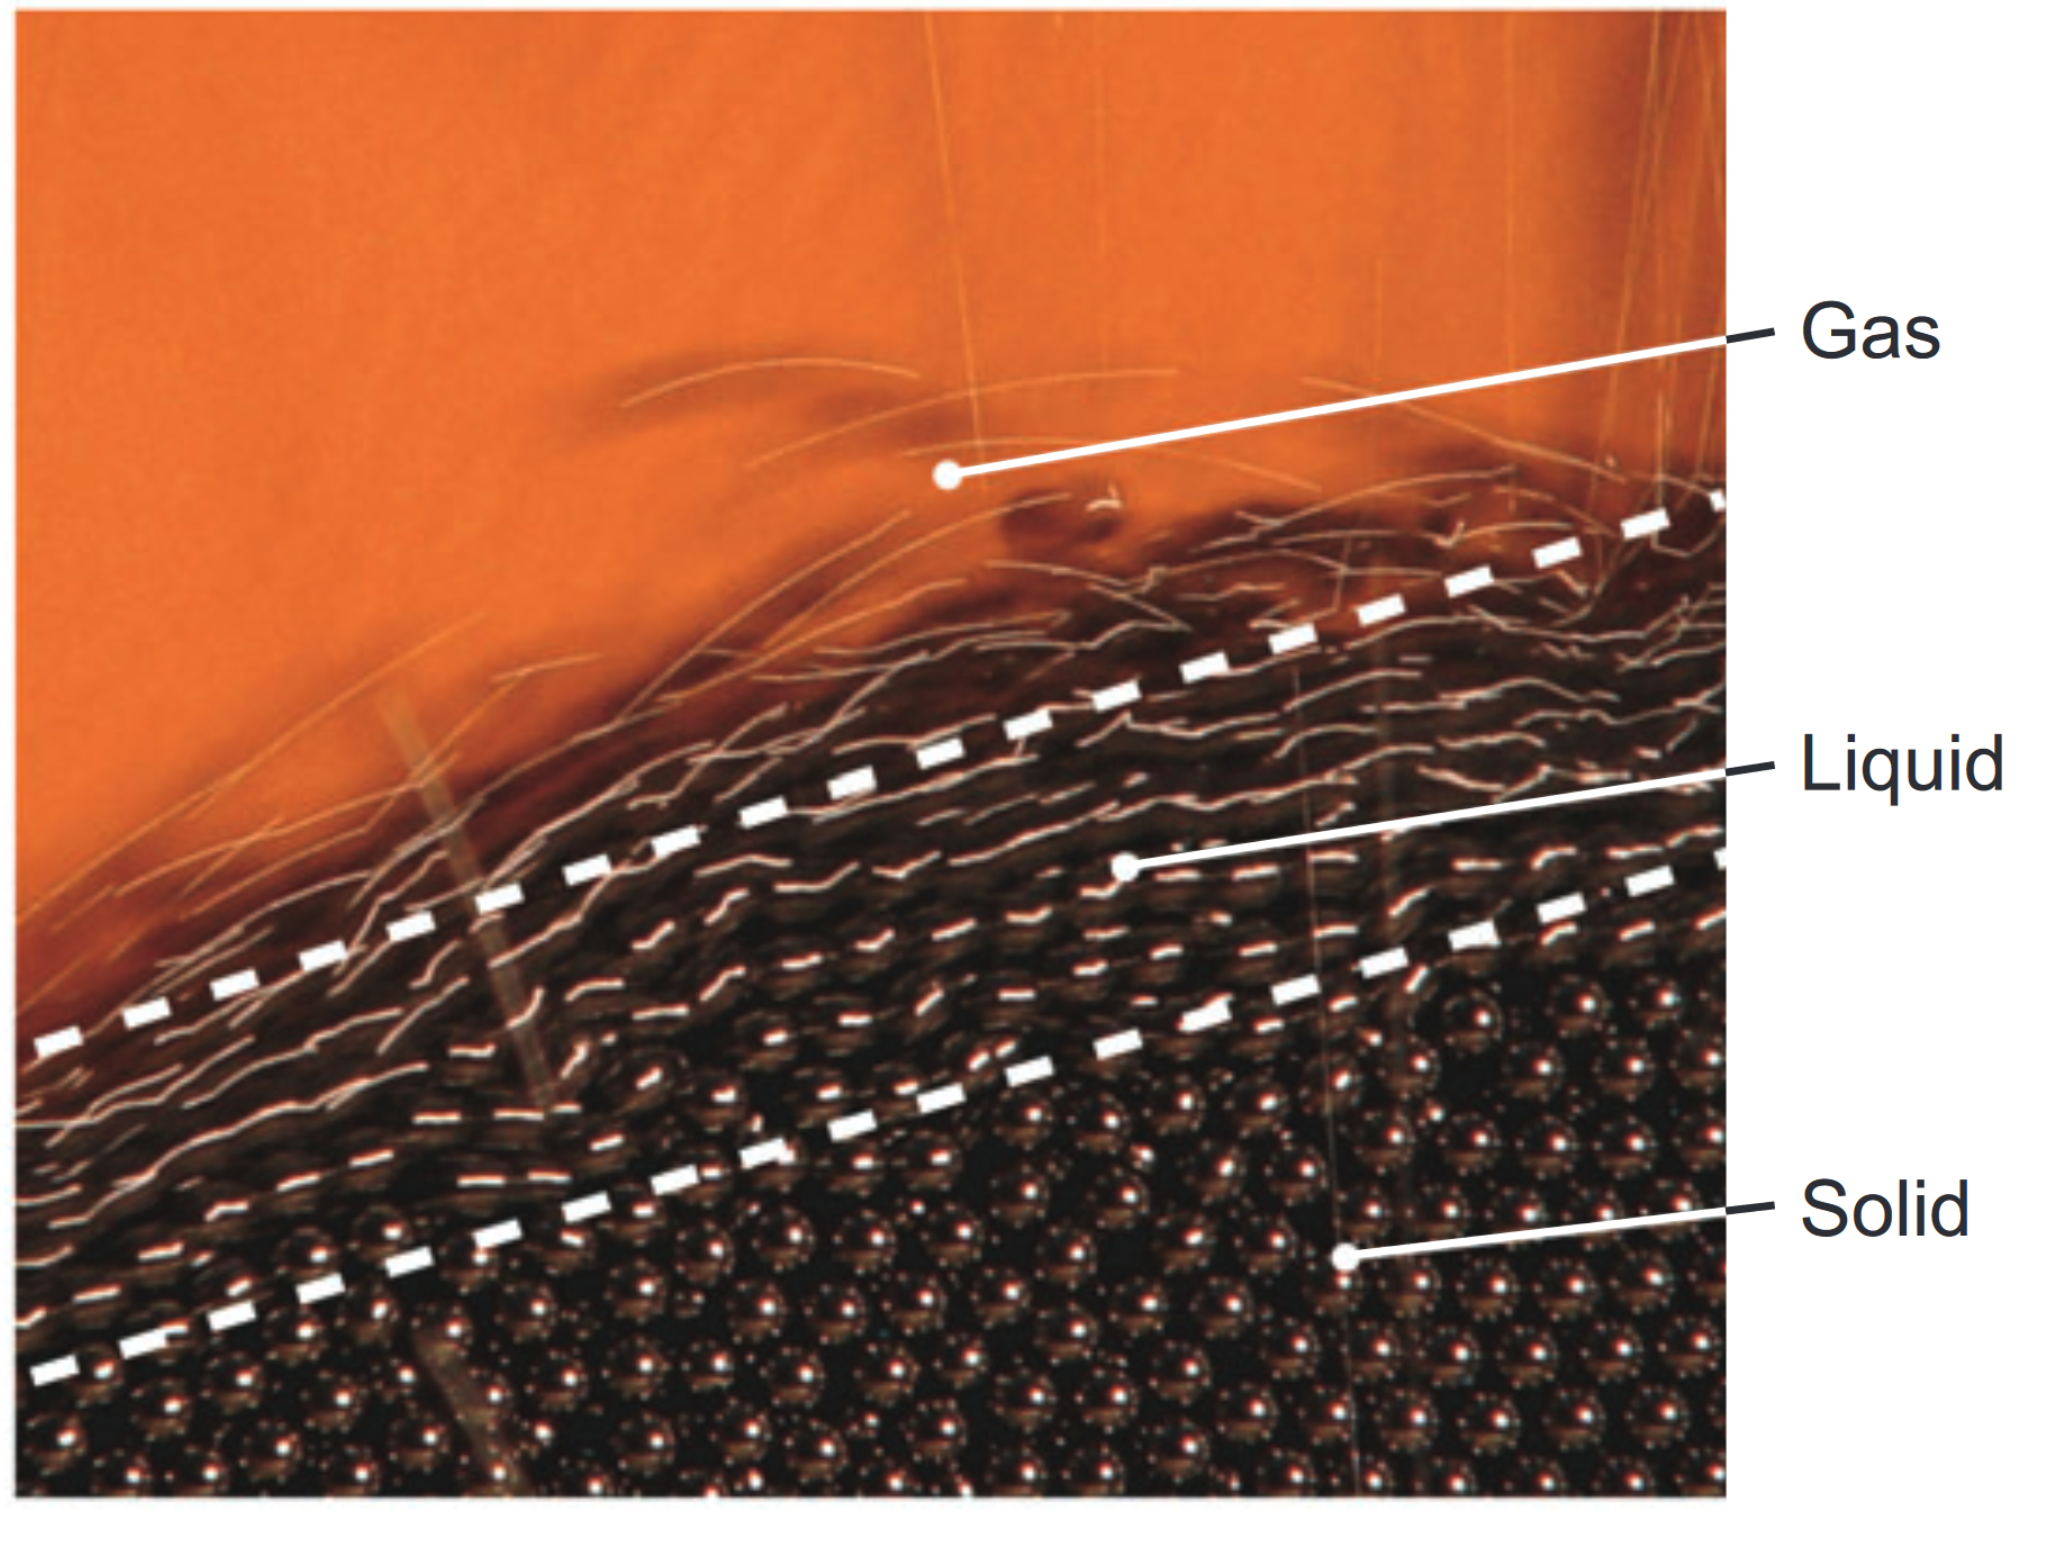
\includegraphics[width=0.5\textwidth]{three_regimes.png}
    \caption{Image de billes d'acier s'écoulant d'un tas. Trois phases de l'écoulement granulaire, se comportant comme un gaz, un liquide ou un solide, peuvent être identifiées.~\cite{forterre_flows_2008}}
\end{figure}

Le régime solide ou frictionnel intervient en particulier en mécanique des sols pour la prédiction de la défaillance des sols pour les applications de génie civil~\cite{Campbell2006}. Dans ce cas, le critère de rupture de Mohr-Coulomb~\cite{Juvinal1991}, accompagné d'une règle de flux de la plasticité des métaux, est suffisant pour décrire le comportement de l'écoulement granulaire comme un processus continu, sans prendre en compte l'interaction des grains individuels. La loi est alors paramétré par des quantités interprétables : l'angle de friction interne, la cohésion, ainsi que l'angle de dilatation. La loi de Drucker-Prager~\cite{Drucker1952}, version lissée du critère de Mohr-Coulomb est également couramment utilisée.


Le régime liquide ou d'écoulement est principalement décrit à l'aide de lois rhéologique. Les travaux récents convergent vers une loi de comportement viscoplastique défini sous le nom de loi $\mu(I)$~\cite{gdr_midi_dense_2004,jop_constitutive_2006}. Des simulation du tambour en rotation~\cite{Cortet_2009} ont pu être réalisé et montre une bonne correspondance pour le cas d'écoulement avec surface libre~\cite{chou_cross-sectional_2009}. Toutefois, cette loi trouve certaines limites dans le cas d'écoulement confiné où le coefficient de tassement change et où le mouvement de chaque grain entraîne des modifications significatives dans les chaînes de force. Si la prédiction est bonne au niveau des bords, elle reste toutefois insuffisante au niveau des parois~\cite{Rognon_Miller_Metzger_Einav_2015}.

Finalement le régime gaz ou cinétique correspond au écoulement granulaires dispersés. Ce sont alors des modèles de cinétique des gaz qui sont utilisé pour modéliser le comportement du milieu granulaire~\cite{Ng2008}.

\subsection*{Simulation de l'écoulement granulaire au sein d'un tambour en rotation}~\label{sec:methode_resolution}

Dans le tambour en rotation l'ensemble des trois zones d'écoulement sont présentes. En fonction du nombre de Foudre, divers régimes d'écoulement apparaissent~\cite{MELLMANN2001251}. Entre autres, on retrouve le glissement, l'avalanche, la cascade, le cataracte, la centrifugation illustrés Figure~\ref{}

\begin{figure}~\label{fig:flow_drum}
    \centering
    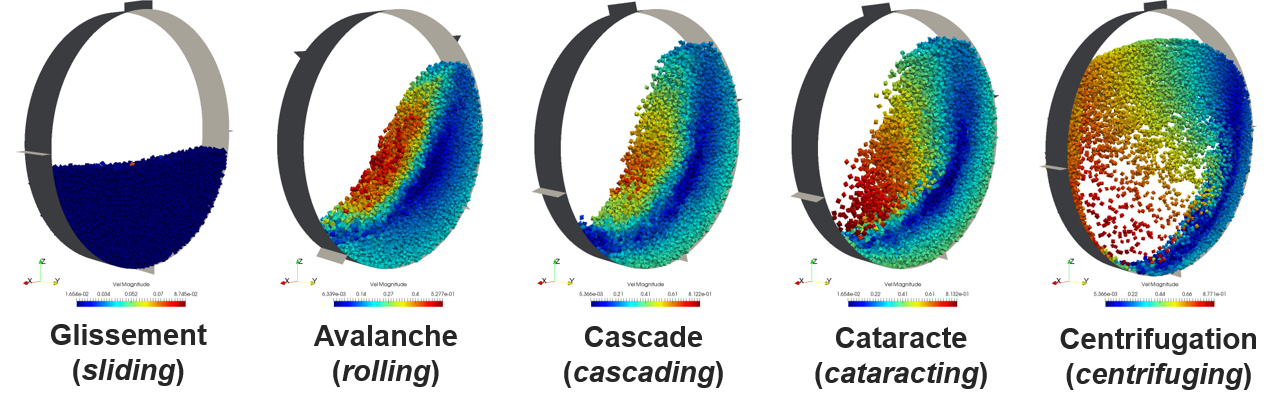
\includegraphics[width=0.8\textwidth]{flows_in_drum.png}
    \caption{Représentation des différents régimes d'écoulement au sein du tambour en rotation avec la méthode DEM.}
\end{figure}

Ces différents régimes déterminent la qualité du mélange, du broyage. C'est en particulier le régime en cascade qui est recherché pour la réduction de taille de grain dans le broyeur à boulets. C'est dans ce régime que la surface libre prend la forme caractéristique d'un \textit{S}.

Outre la difficulté dans la définition de la loi de comportement décrit précédemment, c'est le choix de la modélisation qui est complexe pour ce type de simulation. En effet, ce problème présente un cas d'écoulement en grande transformation, avec une surface libre et nécessitant de tenir compte des interactions avec une paroi mobile voir des corps broyants.

Ce sont d'abord des lois empiriques ou analytiques qui ont été proposées dans la littérature~\cite{Ding2001,Boateng1998,Nicholas2001} mais ceux-ci sont généralement dépend du problème traité, simplifié et ne permettent donc pas une bonne généralisation.

Les méthodes de simulation ce sont à la fois portées sur des représentations continues ou discrète du milieu.

Les méthodes discrètes vont conserver une représentation particulaire du milieu en considérant un jeu de particules en équilibre. Introduite en 1979 par Cundall and Strack~\cite{cundall_discrete_1979}, la méthode des éléments discrets (DEM) a été utilisé pour la première fois pour la modélisation du tambour en rotation par Mishra and Rajamani~\cite{Mishra1992}. Ces méthodes ont l'avantage de pouvoir représenter les différents régimes d'écoulement granulaire, le mélange ou bien les phénomènes de ségrégation. On trouve également des extensions pour prendre en compte la fragmentation~\cite{orozco:hal-02409236}. Malgré ces différents avantages, la méthode DEM est très coûteuse en temps de calcul, en particulier lors de la détection des contacts. C'est d'autant plus le cas pour la simulation du tambour qui fait intervenir des grains de l'ordre du minimètre pour décrire un écoulement de l'ordre du mètre. Les grains simulés sont alors agrandi, représentés avec des géométries plus régulière et lisse, pour permettre un temps de calcul acceptable.
De plus, la DEM nécessite l'introduction d'un terme dissipatif qu'il est souvent difficile à justifier physiquement.

De l'autre côté, les méthodes continues représentent le milieu granulaire comme un milieu continu. Le système est gouverné par les équations de conservation de masse et de quantité de mouvement. Ce type d'approche est plus à même de représenter des écoulements à grande échelle.

Dans cette famille de méthode on retrouve des méthodes qui utilise un maillage pour discrétiser les différents champs approchés. En particulier, on retrouve des méthodes utilisés en dynamique des fluides comme la méthode des volumes finis~\cite{Santos2013,arseni_granular_2020} ou bien en mécanique des solide avec des extensions de la méthodes des éléments finis comme les éléments finis eulérien~\cite{ZHENG2015361}. Si ces méthodes sont relativement plus efficaces en terme de calcul que la méthode DEM, elle ne sont pas bien adaptée aux problèmes avec des interfaces matérielles mobiles et des surfaces libres en raison de leur nature eulérienne.

Finalement, une autre classe de méthode continue a été plus récemment utilisées pour traiter des problèmes impliquant des grandes transformations, des écoulements à surface libre et des problèmes à géométries complexes. Il s'agit des méthodes sans maillage continues. Contrairement au méthode eulérienne à maillage fixe, ces méthodes dites lagrangiennes, utilise un ensemble de \textit{particulaire} comme support de discrétisation qui vont évoluer en suivant l'écoulement. De cette manière, ces méthodes ne peuvent pas souffrir de distorsion de maillage et elle sont beaucoup moins sensible à la dissipation lors de la phase d'advection. Elle permette de prendre en compte d’un mélange en affectant à chaque particules différentes particules et traite le problème de surface libre nativement. Une des plus connues est la méthode SPH (\textit{Smoothed Particle hydrodynamics}), où chaque particule transporte des quantités matérielles ainsi qu'une fonction noyau pour interpoler et discrétiser les champs continus et leurs opérateurs différentiels. Cette méthode a été utilisée pour simuler le tambour en rotation à l'aide d'une loi $\mu(I)$ couplé à une surface de charge de Drucker-Prager~\cite{zhu_lagrangian_2022}. Une autre méthode, particulièrement utilisé en mécanique des solides, est la méthode MPM (\textit{Material Point Method}). Cette dernière est une extension de la méthode PIC \textit{Particle In Cell}. Cette méthode hybride a été largement utilisée pour les écoulement granulaire~\cite{KUMAR201794} ainsi que pour la simulation du tambour en rotation~\cite{zuo_numerical_2020, chandra_nonconforming_2021} et a pu être comparé à la fois à la méthode DEM et l'expérimental pour étudier le mélange. Cependant, contrairement aux méthodes avec maillage, on perd en efficacité de calcul soit par des étapes de recherche de plus proches voisin en SPH, ou part le calcul des transfers grille/particules en MPM.

Finalement, bien que le sens physique ne soit pas le même entre méthodes discrètes et continues, il existe une prédominance des méthodes sans maillages dites particulaires pour traiter le problème de l'écoulement dans un tambour en rotation comme illustré Figure~\ref{fig:simu_granulaire}.

\begin{figure}[h]
    \centering
    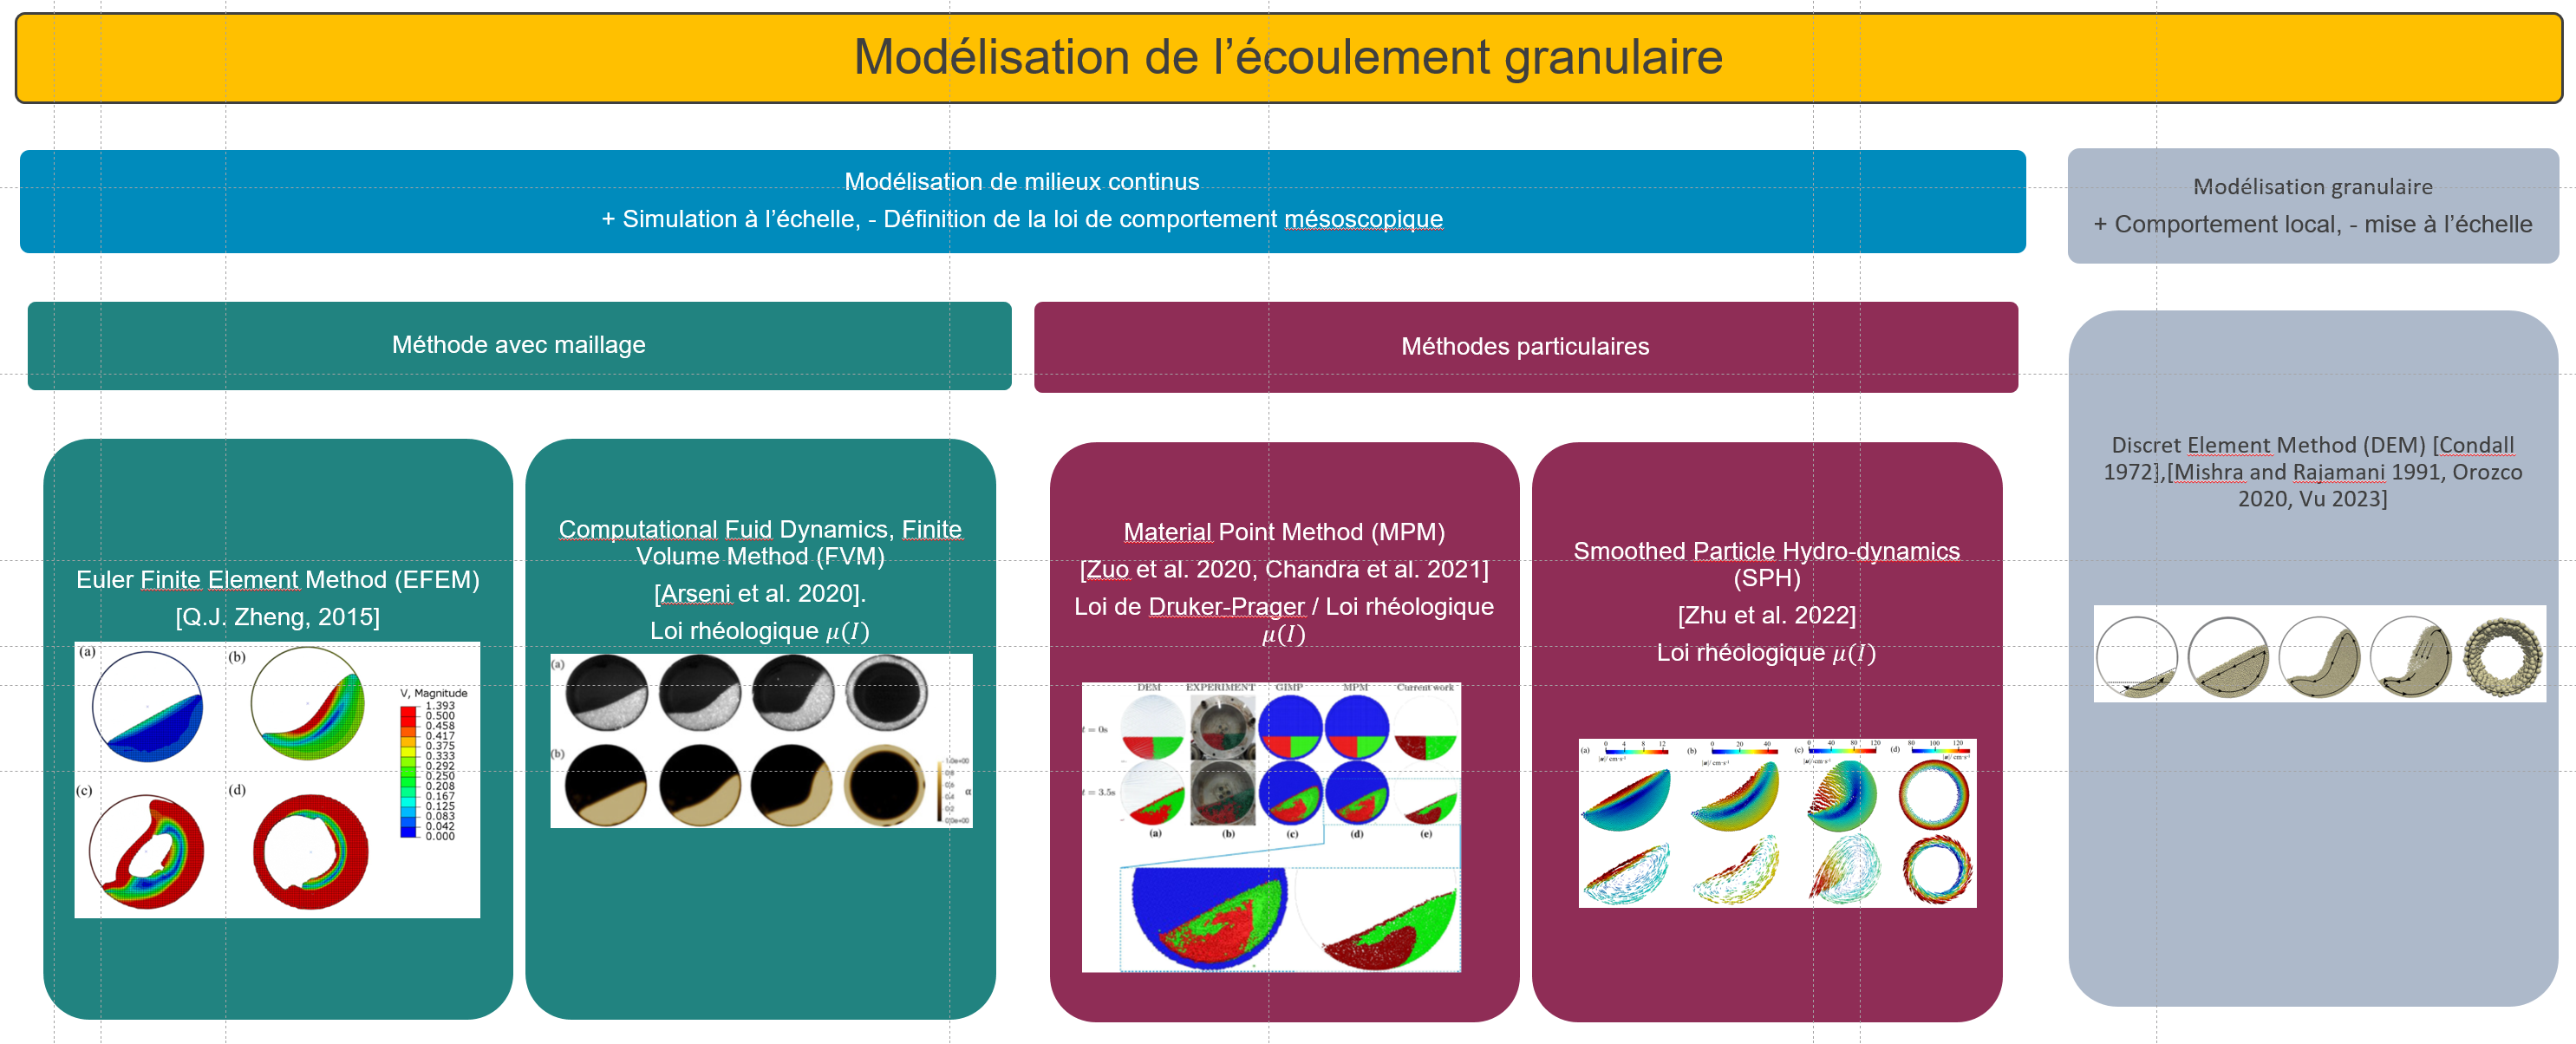
\includegraphics[width=\textwidth]{simulation_granulaire.png}
    \caption{Catégorisation des simulations de l'écoulement granulaire au sein d'un tambour en rotation.}~\label{fig:simu_granulaire}
\end{figure}

\subsection*{Mesures appliquées au tambour en rotation}~\label{sec:mesures}

Outre l'utilisation d'outils de simulation, la validation et la compréhension du procédé se voient renforcés par l'utilisation accrue de méthodes de mesure durant la phase de fonctionnement.

Ces données sont de différents types. D'une part, des données issues de l'imagerie~\cite{jarray_wet_2019,Adepu}. Celles-ci nous permette de mesurer des mesures de champ de vitesse capturées à travers la face avant d'un hublot transparent grâce à la méthode \textit{Particle Image Velocimetry} (PIV), de mesurer le ou bien de post traiter des grandeurs caractéristiques comme l'angle de repos dynamique ou de mesurer des indices de mélange.

D'autre part, des mesures acoustiques du broyeur peut révéler des informations sur divers aspects du processus, tels que les conditions de fonctionnement, les anomalies potentielles, ou encore l'usure des éléments du broyeur~\cite{Owusu, almond}.

On trouve également dans la littérature l'usage de mesure vibratoire ou de jauges de contraintes sur la paroi afin de déterminer la position du corps broyant~\cite{Davey, tano_2005}, des données issues du moteur~\cite{pedrayes_frequency_2017} ou bien l'instrumentation des boulets~\cite{Wang} (ce qui difficilement réalisable dans notre situation où la matière est contaminée).

Le laboratoire expérimental SA3E a instrumenté une maquette de broyeur dont des acquisitions sont représentées sur la Figure~\ref{fig:mesures}.

\begin{figure}[h]
    \centering
    \begin{subfigure}[b]{0.3\textwidth}
        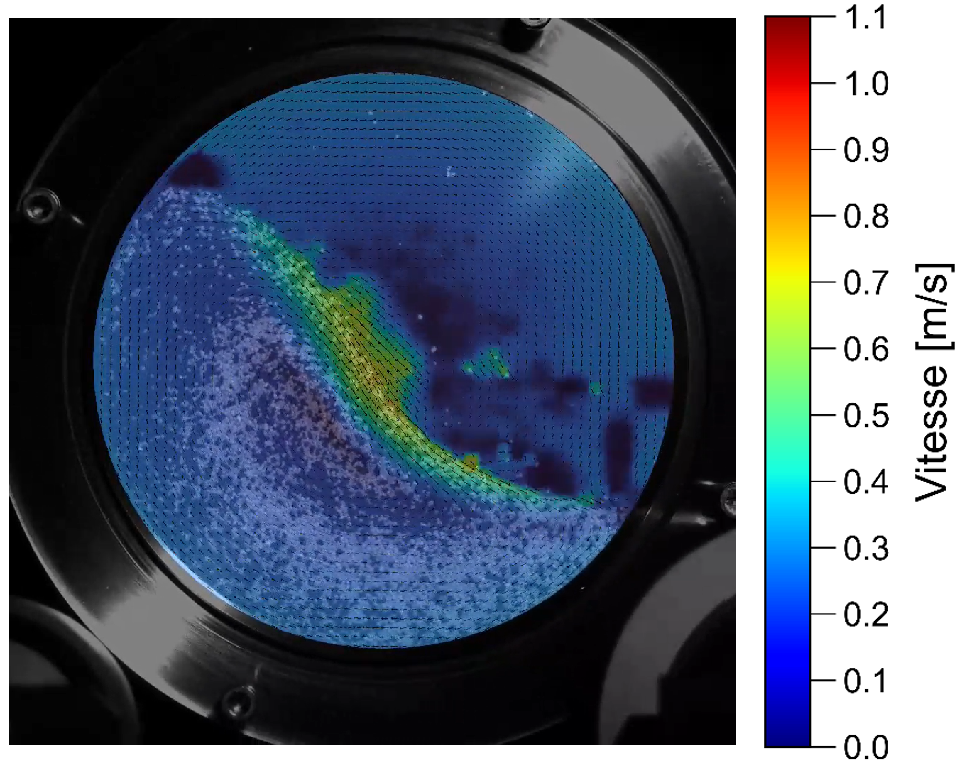
\includegraphics[width=\textwidth]{mesure_pic.png}
        \caption{particule Image Velocimetry}
    \end{subfigure}
    \hfill
    \begin{subfigure}[b]{0.3\textwidth}
        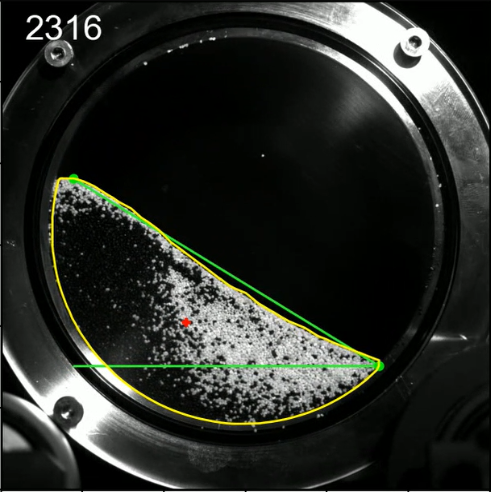
\includegraphics[width=\textwidth]{mesure_theta.png}
        \caption{angle de repos dynamique}
    \end{subfigure}
    \hfill
    \begin{subfigure}[b]{0.3\textwidth}
        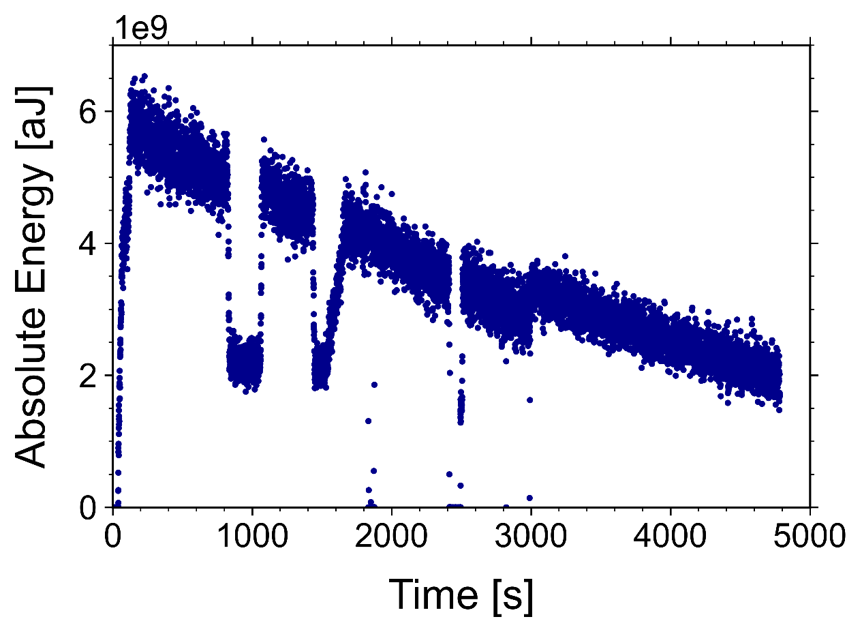
\includegraphics[width=\textwidth]{mesure_ea.png}
        \caption{mesures electro-acoustique}
    \end{subfigure}
    \caption{Exemples d'acquisition sur la maquette du broyeur à boulets au laboratoire du SA3E.}~\label{fig:mesures}
\end{figure}

Une large gamme de mesures sont donc disponibles. Cependant, ces données mesurées ne permettent que d'avoir une représentation partielle et bruitée de l'état réel du broyage et du mélange. De plus, La qualité des résultats analysée reste néanmoins très variable. En effet, l'interprétabilité de bon nombre ce fait au travers de méthode de corrélation et non pas via des approches inductives.

Finalement, les données mesurées que nous possédons ne représentent qu'une vue brute et partielle de l'état réel, tandis que les données simulées de cet état sont sujettes à des erreurs de modélisation. Ainsi, nous souhaitons trouver un moyen d'améliorer notre connaissance des processus en tenant compte à la fois de la simulation et des mesures expérimentales.

\subsection*{Jumeau numérique}

La notion de jumeau numérique trouve un essor considérable aujourd'hui à l'air où la données n'ont jamais été aussi présente. Le potentiel grandissant de la \textit{Big Data}, \textit{l'Internet Of Things}, le calcul haute performance (HPC) mais aussi de l'intelligence artificiel (IA) et en particulier l'apprentissage profond ouvre la voie à de nouveaux outils. Bien que sur toutes les lèvres, on trouve difficilement une définition univoque de ce paradigme.
En effet, le jumeau numérique peut être tour à tour vu comme un réplique haute fidélité capable d'émuler un système réel~\cite{noauthor_digital_nodate}, ou bien comme un modèle dynamique qui est capable d'être mis à jour avec les données de son pendant physique au long de son cycle de vie afin d'apporter une aide à la décision~\cite{AIAA2020}. Pour éviter toute confusion la distinction est souvent faite entre \textit{Virtual Twin}, \textit{Predictive Twin}, ou encore \textit{Twin Projection}~\cite{Kvamsdal}.

En définitif, le jumeau numérique n'est autre qu'un modèle, et répond au principe d'utilité énoncé par Box~\cite{box1979}: \textit{All models are wrong, some are useful}.

Le jumeau numérique pour l'étape de fabrication du combustible peu donc répondre à différents niveaux d'usages comme :
\begin{itemize}
    \item avoir une meilleure compréhension du procédé ;
    \item avoir une prédiction fidèle de l'état du système ;
    \item proposer une optimisation des paramètres de contrôle ;
    \item surveiller l'état du procédé dans une optique de maintenance prédictive ;
    \item contrôler la qualité du produit.
\end{itemize}

Finalement, le jumeau numérique peut être formalisé mathématiquement sous la forme d'un modèle graphique probabiliste proposée par Kapteyn et al.~\cite{kapteyn_probabilistic_2021}.
Elle permet de relier de bout en bout les flux de données entre capteur, et modèle numérique, mais aussi avec les paramètres de contrôle et de récompense. La représentation graphique du jumeau numérique du broyeur est présentée en Figure~\ref{fig:graph_dt}.

\begin{figure}[h]
    \centering
    \begin{subfigure}{0.44\textwidth}
        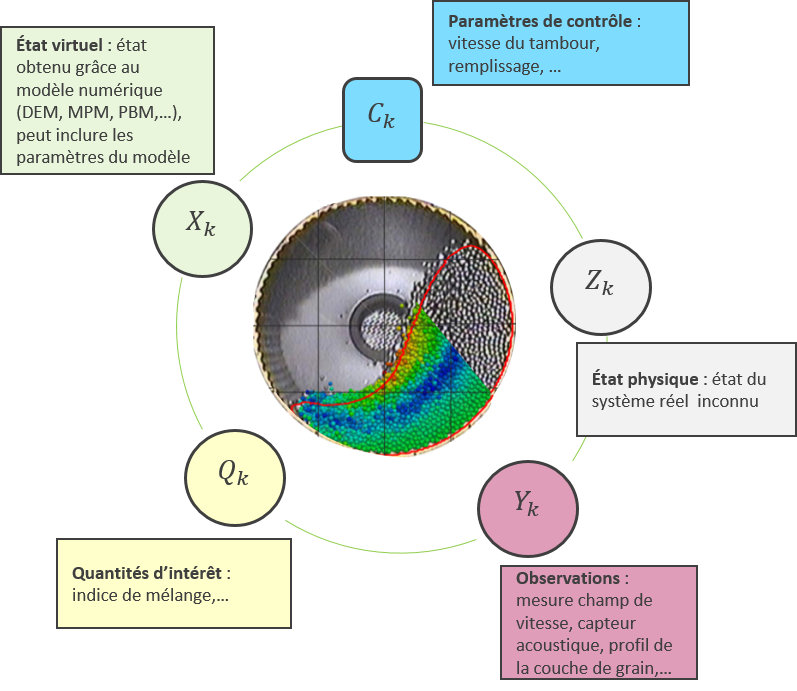
\includegraphics[width=\textwidth]{dt_broyeur.png}
    \end{subfigure}
    \hfill
    \begin{subfigure}{0.55\textwidth}
        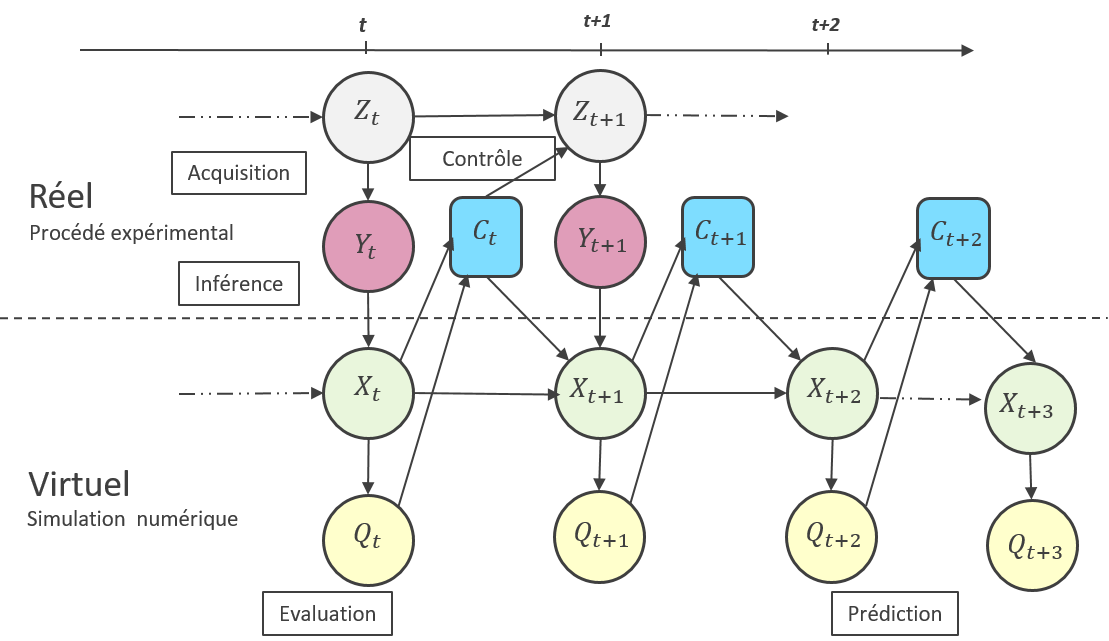
\includegraphics[width=\textwidth]{dt_seq.png}
    \end{subfigure}
    \caption{Variables et représentation graphique du jumeau numérique du broyeur à boulets.}~\label{fig:graph_dt}
\end{figure}

D'une part, on représente bien l'entité réel qui n'est connue qu'au travers des observations présentées Section~\ref{sec:mesures}. Mathématique il s'agit d'un modèle de Markov caché. D'autre part, on retrouve le modèle virtuel qui permet d'avoir accès aux variables d'intérêt et de prédire l'évolution de l'état du système à l'aide des modèles physiques comme présenté en Section~\ref{sec:methode_resolution}
Finalement, on remarque le lien d'inférence qui permet de relier les observations et avec l'état virtuel du système. Fondamentalement, ce sont les méthode d'inférence bayésienne, et l'assimilation de données qui sont utilisés à cette étape.
Le modèle probabiliste permet ainsi d'intégrer dans la construction du jumeau numérique la notion de quantification d'incertitude.




